Como ya se explicó en la sección \textit{explicación}, el peor caso es aquel en el que todos los vértices tienen grado 2.\\
Para generar los casos de prueba se escribió un programa generador (adjunto con el tp). El mismo acepta dos parámetros de entrada $min$ y $max$, siendo la cantidad de vértices mínima y 
máxima respectivamente. El programa entonces genera un archivo con 1 grafo por cada n (con el formato adecuado). El tiempo se midió en nanosegundos por una cuestión de facilidad ya que 
las funciones para ello ya estaban implementadas del tp anterior.\\
Para cada grafo de n nodos, ejecutamos la función principal de nuestro programa que calcula si es orientable o no 5 veces, quedándonos con el mínimo valor de tiempo, ya que cualquier 
cosa que afecte a la ejecución del programa (interrupciones del sistema operativo) sólo lo incrementará.\\

\begin{center}
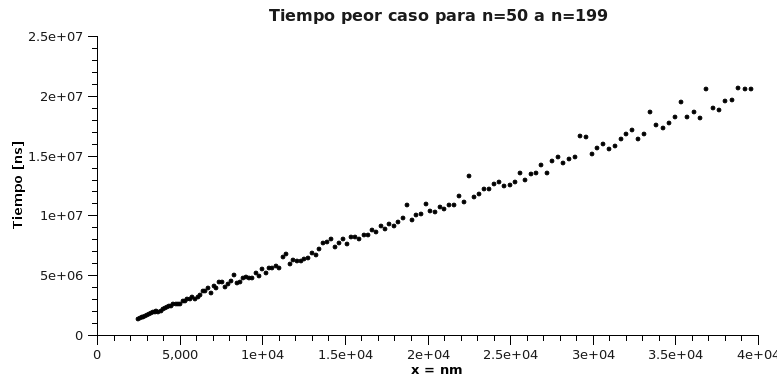
\includegraphics[scale=0.7]{img/ej2/tiempos2.png} 
\end{center}
\begin{center}
 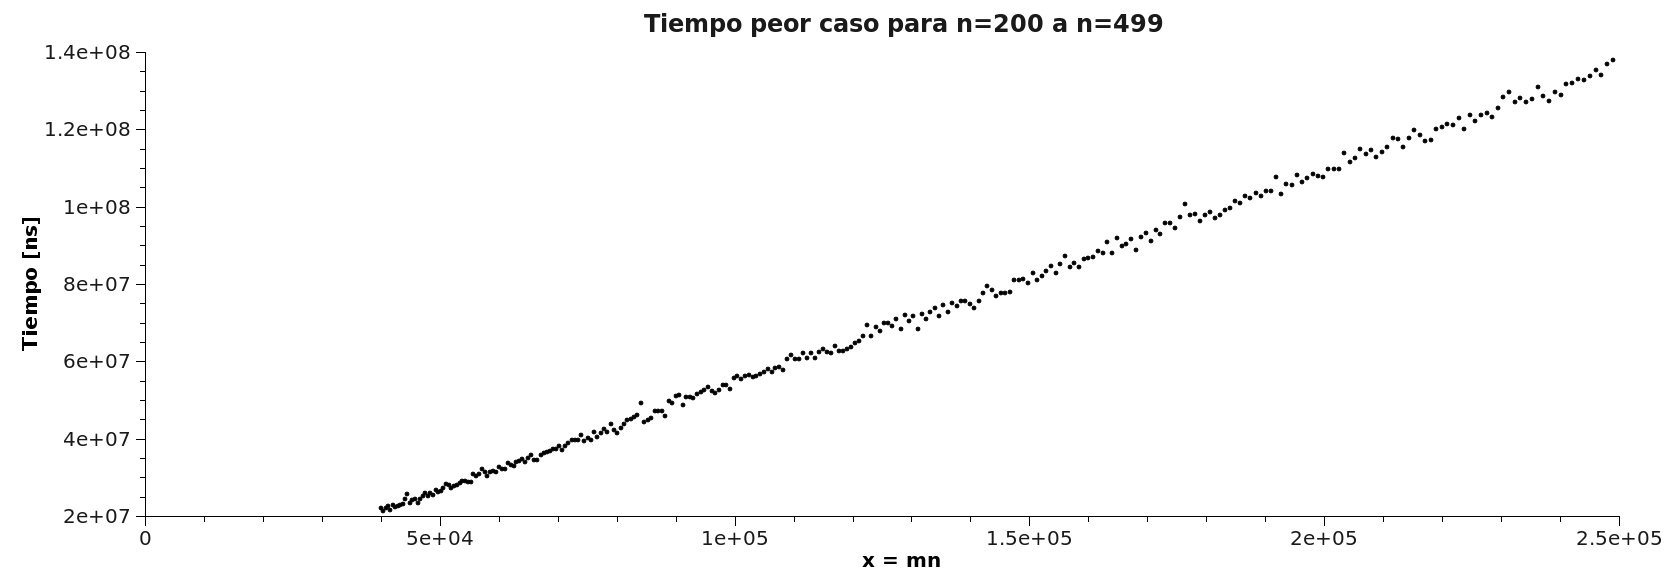
\includegraphics[scale=0.4]{img/ej2/tiempos3.png}
\end{center}
